\documentclass{article}
\usepackage{graphicx}
\usepackage{listings}
\usepackage{enumitem}
\usepackage[total={8in, 10.5in}]{geometry}
\usepackage{courier}
\lstset{
  breaklines=true,
  frame=single,
  gobble=16,
  tabsize=4,
  language=bash,
  basicstyle=\small\ttfamily,
}

\author{Iresh Dissanayaka}

\title{Enabling HTTPS Communication for IBM AppConnect Integrations}

\begin{document}
    \maketitle

    \section{Introduction}
    This document is intended to be a guide to secure http communication
    (https) in IBM App AppConnect Enterprise. The document only covers
    enabling https for the http applications hosted in an existing
    integration node setup.

    \section{Quick TLS/SSL Guide}
    \subsection{What it enables?}
    It enables some server or a client (or generally, an entity) to
    authenticate themselves to some other server or a client and encrypt
    the communication. TLS/SSL is what makes http into https.

    \subsection{How does it do that?}
    \begin{itemize}
        \item So there is this pair called public, private key pair.
        \item Those two are just two values (two pieces of data) you may represent as two numbers, strings, stream of bytes, bits, whatever you want to see it as. However, we call them `keys'.
        \item Those two keys have a cool property where you can use the public key to encrypt some data and you can only decrypt it with the corresponding private key and vice versa.
        \item Keep in mind that the private key is never distributed. It's a secret and it's kept private. Public key is simply public.
        \item There's our server too. It can make use of those keys by creating a key pair and distributing the public key to others. Anyone else can encrypt data with the public key and send it to the server and since only the server has the corresponding private key, only the server can decrypt the data. Not even the original sender can decrypt once encrypted. We didn't share any password or sensitive information with other parties. How cool is that?
        \item Well! there's still a problem. How can other parties be sure that they have received actually the server's public and not some hacker's public key of which he/she has the corresponding private key. Who knows, hacker might have intercepted the communication while server was distributing the public key.  Remember this as `Key Distribution Problem'
        \item Welcome certificates and certificate authorties to the party. They solve the aforementioned problem. Side note: A certificate authority has their own private and public key pair.
        \item A certificate authority is a third party trusted by everyone by default. For example: Google (think of something else if you don't trust google)
        \item Ohh! One more thing, there's this thing called digital signatures. It's the digital version of signing a document but more reliable. Think of it this way. Someone can use their private key to sign some data and others can use the corresponding public key to verify that the signature is valid. Therefore the data is guaranteed to be originating from and signed by the private key's owner. That's what signatures do right?
        \item What's a certificate? Certificate is a piece of data which contains a public key and corresponding owner's information and more importantly all that information is signed by a certificate authority
        \item Remember that `Key Distribution Problem'? Remember that a certificate authority is trusted by default? Remember what digital signatures do? Remember that a certificate is signed by a certificate authority? Since, all the parties trust the certificate authority, whatever information signed by the certificate authority is also trusted. Therefore, `Key Distribution Problem' can be solved. Because, even if a hacker does intercept the communication and send their public key, that is not signed by a certificate authority to impersonate the server. So other parties can detect that. Therefore other parties can always verify the original server's public key not get tricked by a hacker to use their public key instead.
        \item One more thing, certificate authority is referred to as a CA in short and they have their own private key and the corresponding certificate which contains the public key. If you are wondering, that certificate is signed by themselves and it is called self signed. After all, we don't need any other party to sign their certificate because we anyways trust them by default.
    \end{itemize}

    \subsection{TLS/SSL Summary}
    There are the client and the server, purpose is to authenticate the server to the client and encrypt further communication. Server has a certificate signed and issued by a CA. Client trusts the CA and all the certificates issued by the CA. Therefore, server certificate is trusted by the client. So the client can authenticate the server. 
    
    \section{Configuring TLS/SSL for an integration node}
    This is the general procedure for configuring TLS/SSL for http communication for an existing integration node. Configuring TLS/SSL is just providing certificates and private keys (along with some parameters) to the intergration node using a standardized way.

    \subsection{Prerequisites}
    \begin{itemize}
        \item Integration node running
        \item Certificate for the integration node and corresponding private key
        \item CA certificate by which integration node certificate has been signed
    \end{itemize}

    \subsection{Procedure outline}
    \begin{enumerate}
        \item Gather the certificate files and the private key in some format. Ex: x509 PEM
        \item Create a keystore to store them (keystore is just a file that contains certificates, private keys and other type of credentials)
        \item Provide the keystore to the integration node so it can access the required certificates and the private key
    \end{enumerate}

    \subsection{Procedure}
    This section describes outlined procudure in detail. Note that the file names here are arbitrary.
    \subsubsection{Gather the required certificate and private key files}
    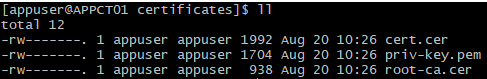
\includegraphics[width=\textwidth,height=\textheight,keepaspectratio]{cert-ls.png}
    \begin{itemize}
        \item \texttt{cert.cer} is the integration node's certificate
        \item \texttt{priv-key.pem}  is the corresponding private key
        \item \texttt{root-ca.cer} is the CA's certificate
    \end{itemize}

    \subsubsection{Create a keystore}
    Idea here is to bundle all three files into a single file called `keystore'.

    \begin{enumerate}[itemsep=4ex]
        \item Verify all three files and their formats
        \begin{enumerate}[itemsep=3ex]
            \item Verify the integration node certificate file.


            The certificate file might be encoded in PEM (regardless of the file extension) or DER binary format. To check whether it is in PEM, run,
            \begin{lstlisting}
                openssl x509 -in cert.cer -subject -noout
            \end{lstlisting}
            If it says something similar to following, it is in PEM.
            \begin{lstlisting}
                subject= /C=LK/ST=WESTERN/L=COLOMBO 3/O=DFCC BANK PLC/OU=IT/CN=esbprod.dfcc.net
            \end{lstlisting}
            else if it says something similar to following, it is probably in DER
            \begin{lstlisting}
                unable to load certificate
                139778153113488:error:0906D06C:PEM routines:PEM_read_bio:no start line:pem_lib.c:707
            \end{lstlisting}
            then run the following to check whether it is DER,
            \begin{lstlisting}
                openssl x509 -inform der -in cert.cer -subject -noout
            \end{lstlisting}
            If it says something similar to following, it is in DER.
            \begin{lstlisting}
                subject= /C=LK/ST=WESTERN/L=COLOMBO 3/O=DFCC BANK PLC/OU=IT/CN=esbprod.dfcc.net
            \end{lstlisting}
            if that results an error as well, something might be wrong. Check your certificate file.

            
            If your certificate file was in DER, convert that to PEM and replace the original file \texttt{cert.cer}, Run,
            \begin{lstlisting}
                openssl x509 -inform der -in cert.cer -outform pem -out cert.pem
                mv cert.pem cert.cer
            \end{lstlisting}

            \item Verify the CA certificate file. Run,
            It is pretty much the same for CA certificate as well.


            The certificate file might be encoded in PEM (regardless of the file extension) or DER binary format. To check whether it is in PEM, run,
            \begin{lstlisting}
                openssl x509 -in root-ca.cer -subject -noout
            \end{lstlisting}
            If it says something similar to following, it is in PEM.
            \begin{lstlisting}
                subject= /DC=net/DC=dfcc/CN=dfcc-ROOTAD-CA-1
            \end{lstlisting}
            else if it says something similar to following, it is probably in DER
            \begin{lstlisting}
                unable to load certificate
                139778153113488:error:0906D06C:PEM routines:PEM_read_bio:no start line:pem_lib.c:707
            \end{lstlisting}
            then run the following to check whether it is DER,
            \begin{lstlisting}
                openssl x509 -inform der -in root-ca.cer -subject -noout
            \end{lstlisting}
            If it says something similar to following, it is in DER.
            \begin{lstlisting}
                subject= /DC=net/DC=dfcc/CN=dfcc-ROOTAD-CA-1
            \end{lstlisting}
            if that results an error as well, something might be wrong. Check your certificate file.


            If your certificate file was in DER, convert that to PEM and replace the original file \texttt{root-ca.cer}, Run,
            \begin{lstlisting}
                openssl x509 -inform der -in root-ca.cer -outform pem -out root-ca.pem
                mv root-ca.pem root-ca.cer
            \end{lstlisting}

            \item Verify the private key file. Run,
            \begin{lstlisting}
                openssl rsa -in priv-key.pem -check -noout
            \end{lstlisting}
            Example output:
            \begin{lstlisting}
                RSA key ok
            \end{lstlisting}

            \item Verify that the certificate and the private key match. Run,
            \begin{lstlisting}
                test $(openssl x509 -in cert.cer -modulus -noout) = $(openssl rsa -in priv-key.pem -modulus -noout) && echo OK
            \end{lstlisting}
            Example output:
            \begin{lstlisting}
                OK
            \end{lstlisting}

        \end{enumerate}

        \item Bundle the integration node's certificate and the corresponding private key to a single \texttt{.pfx} file so they can imported to the keystore that is yet to be created
    \end{enumerate}

\end{document}